\documentclass[border=10pt]{standalone}
\usepackage[svgnames]{xcolor}
\usepackage{amsmath}
\usepackage{pgfplots}
\pgfplotsset{compat=newest}
\usepackage[sfdefault]{FiraSans}
\usepackage{FiraMono}
\renewcommand*\familydefault{\sfdefault}
\begin{document}
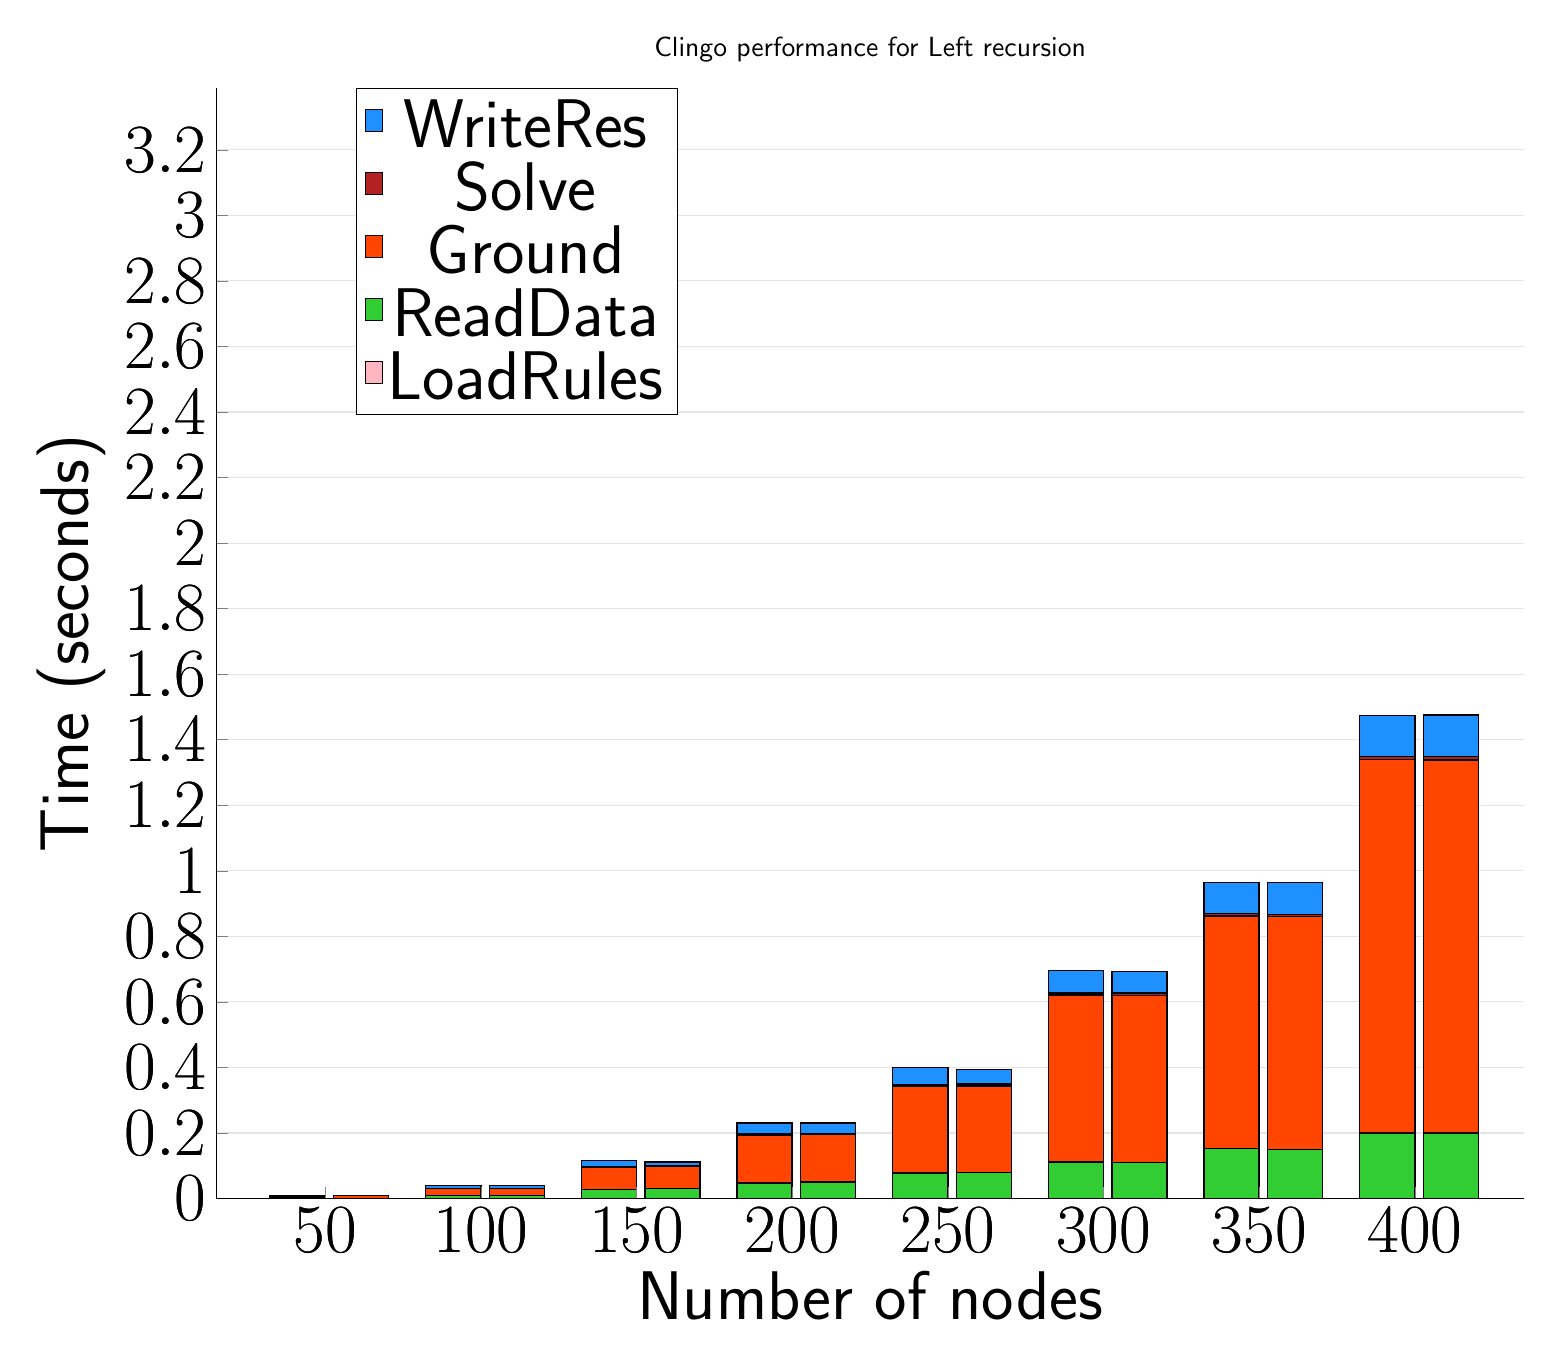
\begin{tikzpicture}
\begin{axis}[
   ybar stacked,
   title={Clingo performance for Left recursion},
   bar shift=-10pt,
   width=1.5\textwidth,
   bar width=0.7cm,
   ymajorgrids, tick align=inside,
   major grid style={draw=gray!20},
   xtick=data,
   ymin=0, ymax=3.3890000581741333,
   axis x line*=bottom,
   axis y line*=left,
   enlarge x limits=0.1,
   legend style={
       at={(0.23, 1)},
       anchor=north,
       legend columns=1,
       font=\Huge,
   },
   ylabel={Time (seconds)},
   xlabel={Number of nodes},
   label style={font=\Huge},
   tick label style={font=\Huge},
]
\addlegendimage{fill=DodgerBlue, draw=black, line width=0.2pt}
\addlegendentry{WriteRes}
\addlegendimage{fill=FireBrick, draw=black, line width=0.2pt}
\addlegendentry{Solve}
\addlegendimage{fill=OrangeRed, draw=black, line width=0.2pt}
\addlegendentry{Ground}
\addlegendimage{fill=LimeGreen, draw=black, line width=0.2pt}
\addlegendentry{ReadData}
\addlegendimage{fill=LightPink, draw=black, line width=0.2pt}
\addlegendentry{LoadRules}
\addplot +[fill=LightPink, draw=black, line width=0.5pt] coordinates {
    (50, 0.0)
    (100, 0.0)
    (150, 0.0)
    (200, 0.0)
    (250, 0.0)
    (300, 0.0)
    (350, 0.0)
    (400, 0.0)
};
\addplot +[fill=LimeGreen, draw=black, line width=0.5pt] coordinates {
    (50, 0.0029999971389770507)
    (100, 0.010000014305114746)
    (150, 0.02799997329711914)
    (200, 0.04799997806549072)
    (250, 0.07799999713897705)
    (300, 0.11099989414215088)
    (350, 0.15199999809265136)
    (400, 0.2)
};
\addplot +[fill=OrangeRed, draw=black, line width=0.5pt] coordinates {
    (50, 0.0029999971389770507)
    (100, 0.020000004768371583)
    (150, 0.06800000667572022)
    (200, 0.14600000381469727)
    (250, 0.26599998474121095)
    (300, 0.5099999904632568)
    (350, 0.7100000143051147)
    (400, 1.1389999866485596)
};
\addplot +[fill=FireBrick, draw=black, line width=0.5pt] coordinates {
    (50, 0.0009999990463256836)
    (100, 0.0)
    (150, 0.0)
    (200, 0.0029999971389770507)
    (250, 0.004000020027160644)
    (300, 0.005999994277954101)
    (350, 0.006999993324279785)
    (400, 0.009999990463256836)
};
\addplot +[fill=DodgerBlue, draw=black, line width=0.5pt] coordinates {
    (50, 0.0029999971389770507)
    (100, 0.009999990463256836)
    (150, 0.020000004768371583)
    (200, 0.03300001621246338)
    (250, 0.050999999046325684)
    (300, 0.06900017261505127)
    (350, 0.09600000381469727)
    (400, 0.1250000238418579)
};
\end{axis}
\begin{axis}[
   ybar stacked,
   bar shift=13pt,
   width=1.5\textwidth,
   bar width=0.7cm,
   ymajorgrids, tick align=inside,
   major grid style={draw=none},
   xtick=data,
   ymin=0, ymax=3.3890000581741333,
   axis x line*=none,
   axis y line*=none,
   enlarge x limits=0.1,
   label style={font=\Huge},
   tick label style={font=\Huge},
]
\addplot +[fill=LightPink, draw=black, line width=0.5pt] coordinates {
    (50, 0.0)
    (100, 0.0)
    (150, 0.0)
    (200, 0.0)
    (250, 0.0)
    (300, 0.0)
    (350, 0.0)
    (400, 0.0)
};
\addplot +[fill=LimeGreen, draw=black, line width=0.5pt] coordinates {
    (50, 0.0)
    (100, 0.009999999999999997)
    (150, 0.030000000000000006)
    (200, 0.049999999999999996)
    (250, 0.07999999999999999)
    (300, 0.11000000000000001)
    (350, 0.15)
    (400, 0.19999999999999998)
};
\addplot +[fill=OrangeRed, draw=black, line width=0.5pt] coordinates {
    (50, 0.009999999999999997)
    (100, 0.020000000000000007)
    (150, 0.06799999999999999)
    (200, 0.14699999999999996)
    (250, 0.263)
    (300, 0.5099999999999999)
    (350, 0.71)
    (400, 1.1380000000000001)
};
\addplot +[fill=FireBrick, draw=black, line width=0.5pt] coordinates {
    (50, 0.0)
    (100, 0.0)
    (150, 0.001999999999999999)
    (200, 0.0)
    (250, 0.006000000000000005)
    (300, 0.007000000000000006)
    (350, 0.007000000000000006)
    (400, 0.010999999999999944)
};
\addplot +[fill=DodgerBlue, draw=black, line width=0.5pt] coordinates {
    (50, 0.0)
    (100, 0.009999999999999995)
    (150, 0.012000000000000014)
    (200, 0.03300000000000001)
    (250, 0.044999999999999984)
    (300, 0.06599999999999995)
    (350, 0.09699999999999998)
    (400, 0.12700000000000006)
};
\end{axis}
\end{tikzpicture}

\end{document}
